\documentclass[12pt]{article}
\usepackage{ryblatex}
\usepackage{extramarks}

\title{SUMS Proofs Workshop: Fall}
\author{}
\date{\today}

% Comment out to add in solutions.
\usepackage{environ}
\RenewEnviron{proof}{}

% Uncomment to add space between problems.
% \usepackage{etoolbox}
% \usepackage{needspace}
% \newlength{\problemsep}
% \setlength{\problemsep}{16\baselineskip}
% \AtBeginEnvironment{problem}{\Needspace*{16\baselineskip}}
% \AtEndEnvironment{problem}{\par\vspace{\problemsep}}

\begin{document}

\section*{SUMS Proofs Workshop: Fall}

Note: Problems marked with (*) are difficult. (**) indicates \emph{very difficult}.

\subsection*{Starter Problems}

\begin{problem}
Prove that $0$ divides an integer $a$ if and only if $a=0$.

\begin{proof}
($\Rightarrow$) If $0$ divides $a$, there exists $k\in\mathbb{Z}$ with $0\cdot k=a$. Hence $a=0$.

($\Leftarrow$) If $a=0$, then $0 = 0\cdot k$ for any $k\in\mathbb{Z}$, so $0$ divides $a$.
\end{proof}
\end{problem}

\begin{problem}
Prove that there do not exist integers $m$ and $n$ such that $14m+21n=100$.

\begin{proof}
Suppose integers $m,n$ satisfy $14m+21n=100$. Factor $7$: $7(2m+3n)=100$, so $2m+3n=100/7$, which is not an integer. This is a contradiction.
\end{proof}
\end{problem}

\begin{problem}
Prove that $n^2$ odd implies that $n$ is odd.

\begin{proof}
We prove the contrapositive: if $n$ is even then $n^2$ is even. If $n=2k$ for some $k\in\mathbb{Z}$ then $n^2=(2k)^2=4k^2=2(2k^2)$ is even. So if $n^2$ is odd, $n$ cannot be even, so $n$ is odd.
\end{proof}
\end{problem}

\begin{problem}
Show that $\sqrt{2}$ is irrational.

\begin{proof}
Suppose $\sqrt{2}\in\mathbb{Q}$ so $\sqrt{2}=\frac{a}{b}$ in lowest terms with $a,b\in\mathbb{Z}$. Squaring gives $2b^2=a^2$, so $a^2$ is even and hence $a$ is even: $a=2k$. Then $2b^2=4k^2$, so $b^2=2k^2$ and $b$ is even. Thus both $a$ and $b$ are even, contradicting the assumption that the fraction was reduced and in lowest terms. Therefore $\sqrt{2}$ is irrational.
\end{proof}
\end{problem}

\begin{problem}
Show that $1^2+2^2+3^2+\cdots+n^2 = \dfrac{n(n+1)(2n+1)}{6}$ for every positive integer $n$.

\begin{proof}
Base case $n=1$: $1^2 = 1 = \frac{1\cdot2\cdot3}{6}$. Assume true for $n-1$. Then
\[
    \sum_{k=1}^n k^2 = \frac{(n-1)n(2n-1)}{6} + n^2
    = \frac{2n^3+3n^2+n}{6} = \frac{n(n+1)(2n+1)}{6},
\]
completing the induction.
\end{proof}
\end{problem}

\begin{problem}
For all $n\in\mathbb{N}$ show that $2^n \le 3^n-1$.

\begin{proof}
Base case $n=1$: $2^1=2\le 3^1-1=2$. Assume $2^{n-1}\le 3^{n-1}-1$. Then
\[
    2^n = 2\cdot 2^{n-1} \le 2(3^{n-1}-1) = 2\cdot 3^{n-1}-2.
\]
Since $2\cdot 3^{n-1}-2 \le 3^n-1$ (because $3^n-1 - (2\cdot 3^{n-1}-2) = 3^{n-1}+1>0$), the inequality holds for $n$.
Thus by induction $2^n\le 3^n-1$ for all $n\in\mathbb{N}$.
\end{proof}
\end{problem}

\begin{problem}
Let $n\in\mathbb{Z}$. Suppose there exists $a\in\mathbb{Z}$ such that $n=a^2-a$. Show that $n$ is even.

\begin{proof}
Case 1: $a$ even, $a=2k$. Then $n=4k^2-2k=2(2k^2-k)$ is even.

Case 2: $a$ odd, $a=2m+1$. Then
\[
    n=(2m+1)^2-(2m+1)=4m^2+4m+1-2m-1=2(2m^2+m),
\]
which is even. In either case $n$ is even.
\end{proof}
\end{problem}

\begin{problem}
Let $f:\mathbb{R}\to\mathbb{R}$ be $f(x)=3x^2+2$. Show that this is not injective.

\begin{proof}
Observe $f(1)=3(1)^2+2=5$ and $f(-1)=3(-1)^2+2=5$, so $f(1)=f(-1)$ with $1\neq -1$. Hence $f$ is not injective.
\end{proof}
\end{problem}

\begin{problem}
Let $\sim$ be an equivalence relation on a set $X$. Prove that for all $a,b\in X$, $a\sim b$ if and only if they have equal equivalence classes.

\begin{proof}
($\Rightarrow$) If $a\sim b$ and $x\in[a]$, then $x\sim a$ and by transitivity $x\sim b$, so $x\in[b]$. Thus $[a]\subseteq[b]$. Symmetrically $[b]\subseteq[a]$, so $[a]=[b]$.

($\Leftarrow$) If $[a]=[b]$ then $a\in[a]=[b]$, so $a\sim b$.
\end{proof}
\end{problem}

\begin{problem}
Let $\sim$ be an equivalence relation on a set $X$. Prove that for all $a,b \in X$, 
\begin{align*}
[a]_\sim = [b]_\sim \text{ or } [a]_\sim \cap [b]_\sim = \emptyset.
\end{align*}
You may use the fact $[a]_\sim = [b]_\sim$ iff $a \sim b$ without proof (this is the previous problem!).

\begin{proof}
Let $a, b \in X$. There are two cases to consider.

Case 1: $a \sim b$. Then by the given fact, $[a]_\sim = [b]_\sim$.

Case 2: $a \not\sim b$. Suppose for contradiction $[a]_\sim \cap [b]_\sim \neq \emptyset$. Then $\exists c \in [a]_\sim \cap [b]_\sim$. This means $c \in [a]_\sim$ and $c \in [b]_\sim$, which implies $a \sim c$ and $b \sim c$. By symmetry of $\sim$, we have $c \sim b$. By transitivity of $\sim$, we get $a \sim b$, contradicting our assumption.

Therefore, either $[a]_\sim = [b]_\sim$ or $[a]_\sim \cap [b]_\sim = \emptyset$.
\end{proof}
\end{problem}

\begin{problem}
Prove that
\begin{align*}
1 \cdot 1! + 2 \cdot 2! + 3 \cdot 3! + \cdots n \cdot n! = (n + 1)! - 1.
\end{align*}
Note $n! = n \cdot (n-1) \cdot (n-2) \cdot 2 \cdot 1$.

\begin{proof}
We proceed by induction on $n$.

Base case: When $n = 1$, we have $1 \cdot 1! = 1 \cdot 1 = 1$ and $(1 + 1)! - 1 = 2! - 1 = 2 - 1 = 1$. 

Inductive step: Assume the equation holds for $k \geq 1$, so
\begin{align*}
    1 \cdot 1! + 2 \cdot 2! + \cdots + k \cdot k! = (k+1)! - 1.
\end{align*}
holds. We need to show it holds for $n = k + 1$. Expanding with the induction hypothesis,
\begin{align*}
    1 \cdot 1! + 2 \cdot 2! + \cdots + k \cdot k! + (k+1) \cdot (k+1)! &= ((k+1)! - 1) + (k+1) \cdot (k+1)!\\
    &= (k+1)! - 1 + (k+2-1)(k+1)!\\
    &= (k+1)! - 1 + (k+2)(k+1)! - (k+1)!\\
    &= -1 + (k+2)!\\
    &= (k+2)! - 1
\end{align*}
Thus, the equation holds for $n = k + 1$, completing the proof by induction.
\end{proof}
\end{problem}

\begin{problem}
Define a relation $\sim$ on $\mathbb{N} \times \mathbb{N}$, where $0 \notin \mathbb{N}$, and
\begin{align*}
(a,b) \sim (c,d) \iff ad = bc.
\end{align*}
Prove that $\sim$ is an equivalence relation.

\begin{proof}
We need to show that $\sim$ is reflexive, symmetric, and transitive.

Reflexivity: For any $(a,b) \in \mathbb{N} \times \mathbb{N}$, $ab = ba$ by commutativity, so $(a,b) \sim (a,b)$.

Symmetry: If $(a,b) \sim (c,d)$, then $ad = bc$. By commutativity, $bc = cb$ and $ad = da$, so $cb = da$, which means $(c,d) \sim (a,b)$.

Transitivity: Suppose $(a,b) \sim (c,d)$ and $(c,d) \sim (e,f)$. Then $ad = bc$ and $cf = de$. Multiplying the first equation by $f$, $adf = bcf$. Multiplying the second equation by $b$, $bcf = bde$. Therefore, $adf = bde$. Since $d \neq 0$, dividing by $d$ gives $af = be$, so $(a,b) \sim (e,f)$.
\end{proof}
\end{problem}

\begin{problem}
Prove that if $|a + b| > 2$, then $|a| > 1$ or $|b| > 1$, where $a,b \in \mathbb{R}$. 

\begin{proof}
We prove by contrapositive. Suppose $|a| \leq 1$ and $|b| \leq 1$. By the triangle inequality,
\begin{align*}
    |a + b| \leq |a| + |b| \leq 1 + 1 = 2.
\end{align*}
Since this is the contrapositive, we are done.
\end{proof}
\end{problem}

\begin{problem}
Your friend claims that
\begin{align*}
1 + 2 + \cdots + n = \frac{n(n+3)}{2} - 1.
\end{align*}
The base case $n = 1$ holds. Does the claim hold in general? If so prove it, if not disprove it.

\begin{proof}
For $n = 1$, $\nicefrac{1(1+3)}{2} - 1 = 1$, so the base case holds. For $n = 2$, the left side is $1 + 2 = 3$, while the right side is $\nicefrac{2(2+3)}{2} - 1 = \nicefrac{2 \cdot 5}{2} - 1 = 5 - 1 = 4$. Since $3 \neq 4$, the claim is false.
\end{proof}
\end{problem}

\begin{problem}
Suppose $a,b,c \in \Z$. Prove $a^2 + b^2 = c^2$ implies either $a$ or $b$ is even.

\begin{proof}
Suppose for contradiction that $a,b,c \in \mathbb{Z}$ such that $a^2 + b^2 = c^2$ and $a,b$ are odd. So $\exists x,y \in \Z$ such that $a = 2x + 1$ and $b = 2y + 1$. Substituting:
\begin{align*}
    c^2 
    &= (2x + 1)^2 + (2y + 1)^2 \\
    &= 2(2(x^2 + y^2) + 2(x + y) + 1)
\end{align*}
We reach a contradiction, since $(2(x^2 + y^2) + 2(x + y) + 1)$ is odd and thus is not divisible by $2$. Then $\sqrt{c^2}$ cannot be an integer.
\end{proof}
\end{problem}

\begin{problem}
Suppose $k,n$ are natural numbers, excluding 0. Then $k \notdivides n$ if and only if there exist $q,r \in \Z$ with $0 < r < |k|$ such that $n = qk + r$. Hint: Use the division theorem: For any $n, k \in \N$, there exists unique $q,r \in \N$ such that $n = qk + r$ and $0 \leq r < |k|$.

\begin{proof}
By the division theorem, we know for any $n, k \in \N$, there exists unique $q,r \in \N$ such that $n = qk + r$ and $0 \leq r < |k|$. By the definition of being divisible, $k \divides n$ if and only if $\exists x \in \Z$ such that $n = xk$. Therefore, by the division theorem, $k \divides n$ if and only if $r = 0$.
\end{proof}
\end{problem}

\begin{problem}
If $n,m \in \mathbb{N}$, prove that if $m \divides n$ and $n \divides m$ then $n = m$.

\begin{proof}
Since $m \divides n$, $\exists k \in \Z$ such that $km = n$. Similarly $\exists l \in \Z$ such that $ln = m$. Then $n = km = kln$. But then $kl = 1$. Since $m,n$ can only be positive numbers, $k=1$ and $l=1$ so $m = n$.
\end{proof}
\end{problem}

\begin{problem}
For sets $A,B,C$ show that $A \cap (B - C) = (A \cap B) - (A \cap C)$. Is it always true thar $A \cup (B - C) = (A \cup B) - (A \cup C)$?

\begin{proof}
Let \(x \in A \cap (B \setminus C)\). Then \(x \in A\), \(x \in B\), and \(x \notin C\).
Thus \(x \in A \cap B\) and, since \(x \notin C\), also \(x \notin A \cap C\).
Hence \(x \in (A \cap B) \setminus (A \cap C)\).

Conversely, let \(x \in (A \cap B) \setminus (A \cap C)\). Then \(x \in A\), \(x \in B\),
and \(x \notin A \cap C\). Since \(x \in A\), the latter means \(x \notin C\).
Thus \(x \in A \cap (B \setminus C)\).

For the second part, Let \(A = B = C = \{1\}\). Then
\[
A \cup (B \setminus C) = \{1\}, \qquad
(B \setminus C) = \varnothing, \qquad
(A \cup B) \setminus (A \cup C) = \varnothing.
\]
Thus the equality fails.
\end{proof}
\end{problem}

\begin{problem}
(\href{https://math.berkeley.edu/~willij/1a/proof-practice.pdf}{From Berkeley's Intro to Proofs}) Prove that the composition of any two decreasing functions is increasing. Hint:  Given decreasing functions $f$ and $g$, and numbers $x_1 < x_2$, show that $f(g(x_1)) < f(g(x_2))$.

\begin{proof}
Let \(x_1<x_2\). Since \(g\) is strictly decreasing we have \(g(x_1)>g(x_2)\).
Because \(f\) is strictly decreasing, from \(g(x_1)>g(x_2)\) it follows that
\(f(g(x_1))<f(g(x_2))\).
Thus \(x_1<x_2\Rightarrow f(g(x_1))<f(g(x_2))\), so \(f\circ g\) is strictly increasing.
\end{proof}
\end{problem}

\begin{problem}
Prove that if $x$ and $y$ are real numbers, then $\text{max}(x, y) + \text{min}(x, y) = x + y$.

\begin{proof}
There are two cases.

\textbf{Case 1:} \(x\le y\).  
Then \(\max(x,y)=y\) and \(\min(x,y)=x\), so
\[
\max(x,y)+\min(x,y)=y+x=x+y.
\]
\textbf{Case 2:} \(y< x\).  
Then \(\max(x,y)=x\) and \(\min(x,y)=y\), so
\[
\max(x,y)+\min(x,y)=x+y.
\]
In both cases the sum equals \(x+y\), establishing the identity.
\end{proof}    
\end{problem}

\subsection*{Harder Problems}

\begin{problem}
(*) Assume that the following statement is true: if Micah dislikes pineapple pizza then he likes pineapple pizza. Does he like pineapple pizza?

\begin{proof}
Let
\[
    p:\ \text{Micah dislikes pineapple pizza}
\]
The hypothesis is $p\Rightarrow \neg p$. Then we can construct the following truth table:
\begin{center}
    \begin{tabular}{c | c | c }
        p & $\lnot p$ & $p \implies \lnot p$ \\
        \hline
        T & T & T \\
        F & F & T \\
        F & T & T
    \end{tabular}
\end{center}


Constructing the truth table shows the only way $p\Rightarrow \neg p$ can hold is when $p$ is false (otherwise $p$ and $\neg p$ would both be true or both false, impossible). Thus $p$ is false, so $\neg p$ is true, i.e. Micah likes pineapple pizza.
\end{proof}
\end{problem}

\begin{problem}
(*) For functions $f:X\to Y$ and $g:Y\to X$ with $g\circ f=\mathrm{Id}_X$, decide the truth of:
\begin{enumerate}
\item $f$ is surjective.
\item $f$ is injective.
\item $g$ is surjective.
\item $g$ is injective.
\end{enumerate}

\begin{proof}
(1) False. Counterexample: $X=[0,1]$, $Y=[-1,1]$, $f(x)=x$, $g(y)=|y|$. Then $g\circ f=\mathrm{Id}_{[0,1]}$ but $f$ is not onto $[-1,1]$.

(2) True. If $f(a)=f(b)$ then $a=g(f(a))=g(f(b))=b$, so $f$ is injective.

(3) True. For any $x\in X$, let $y=f(x)\in Y$. Then $g(y)=g(f(x))=x$, so $g$ is surjective.

(4) False. Using the example in (1), $g(-1)=g(1)=1$, so $g$ need not be injective.
\end{proof}
\end{problem}

\begin{problem}
(*) Show that $\mathbb{N}$ has the same size as $\mathbb{Z}^+$ (the positive integers).

\begin{proof}
Define $f:\mathbb{N}\to\mathbb{Z}^+$ by $f(x)=x-1$. Its inverse $g(y)=y+1$ satisfies $g(f(x))=x$ and $f(g(y))=y$, so $f$ is a bijection and the sets have the same cardinality.
\end{proof}
\end{problem}

\begin{problem}
(*) Negate the following definitions without using the word "not" or the symbol $\lnot$:
\begin{enumerate}
\item $\forall x \in \mathbb{R} \setminus \mathbb{Q}$, if $x^2 \in S$ then $x^3 \in T$.
\item For all $x,y \in \mathbb{R}$, if $x,y \in \mathbb{Q}$ then $x + y \in \mathbb{Q}$.
\item We say $f : X \to Y$ is continuous at $p \in X$ if $\forall \epsilon > 0$, $\exists \delta > 0$ s.t. $\forall x \in E$ with $d_X(x,p) < \delta$, then $d_Y(f(x),f(p)) < \epsilon$ ($\dagger$).
\item For some $f: X \to Y$, we say $\lim_{x \to p} f(x) = L$ if $\forall \epsilon$, $\exists \delta > 0$ s.t. $\forall x \in X$ with $d_X(x,p) < \delta$, then $d_Y(f(x),L) < \epsilon$ ($\dagger$).
\end{enumerate}

\begin{proof} We write out the negations. 
\begin{enumerate}
    \item $\exists x \in \mathbb{R} \setminus \mathbb{Q}$ such that $x^2 \in S$ and $x^3 \notin T$.
    
    \item $\exists x,y \in \mathbb{R}$ such that $x,y \in \mathbb{Q}$ and $x + y \notin \mathbb{Q}$.
    
    \item We say $f : X \to Y$ is not continuous at $p \in X$ if $\exists \epsilon > 0$ such that $\forall \delta > 0$, $\exists x \in E$ with $d_X(x,p) < \delta$ and $d_Y(f(x),f(p)) \geq \epsilon$.
    
    \item For some $f: X \to Y$, we say $\lim_{x \to p} f(x) \neq L$ if $\exists \epsilon > 0$ such that $\forall \delta > 0$, $\exists x \in X$ with $d_X(x,p) < \delta$ and $d_Y(f(x),L) \geq \epsilon$.
\end{enumerate}
Negations can convoluted, so it's important to work through them methodically.
\end{proof}
\end{problem}

\begin{problem}
(*) Consider the claim "$\mathcal{P}(A \cup B) \subseteq \mathcal{P}(A) \cup \mathcal{P}(B)$." If true, prove it. Otherwise, disprove it. Note that $\mathcal{P}(S)$ indicates the powerset of $S$.

\begin{proof}
The claim is false. We disprove by counterexample. Let $A = \{1\}$, $B = \{2\}$, and $A \cup B = \{1, 2\}$. Then $\{1, 2\} \in \mathcal{P}(A \cup B)$, but $\{1, 2\} \notin \mathcal{P}(A) \cup \mathcal{P}(B)$ because $\{1, 2\} \notin \mathcal{P}(A)$ and $\{1, 2\} \notin \mathcal{P}(B)$ since $\{1\} \notin \mathcal{P}(B)$ and $\{2\} \notin \mathcal{P}(A)$ respectively.
\end{proof}
\end{problem}

\begin{problem}
(*) Define a sequence of numbers by $a_0 = 1$ and $a_{n+1} = 3a_n + 2$. Prove $a_n = 2 \cdot 3^n + 1$. 

\begin{proof}
We use induction on $n$.

Base case: $a_0 = 2 \cdot 3^0 - 1 = 2 - 1 = 1$

Inductive step: Assume $a_k = 2 \cdot 3^k - 1$ for some $k \geq 0$.
Then:
\begin{align*}
    a_{k+1} &= 3a_k + 2\\
    &= 3(2 \cdot 3^k - 1) + 2\\
    &= 2 \cdot 3^{k+1} - 3 + 2\\
    &= 2 \cdot 3^{k+1} - 1
\end{align*}

Therefore, $a_n = 2 \cdot 3^n - 1$ for all $n \geq 0$.
\end{proof}
\end{problem}

\begin{problem}
(*) For sets $A,B,C$, is $(A \setminus B) \cup (B \setminus C) \subseteq A \setminus C$? If true prove it, else disprove it.

\begin{proof}
The claim is false. We provide a counterexample. Let $A = \{1, 2\}$, $B = \{2, 3\}$, and $C = \{2, 4\}$. Then $A \setminus B = \{1\}$ and $B \setminus C = \{3\}$, so $(A \setminus B) \cup (B \setminus C) = \{1, 3\}$. But $A \setminus C = \{1\}$, so $(A \setminus B) \cup (B \setminus C) \not\subseteq A \setminus C$.
\end{proof}
\end{problem}

\begin{problem}
(*) Prove or give a counterexample: $(X \cap Y) \times (Z \cap W) = (X \times Z) \cap (Y \times W)$, for any sets $X,Y,Z,W$.

\begin{proof}
Let $(a,b) \in (X \cap Y) \times (Z \cap W)$. Then $a \in X \cap Y$ and $b \in Z \cap W$, which means $a \in X$, $a \in Y$, $b \in Z$, and $b \in W$. Thus, $(a,b) \in X \times Z$ and $(a,b) \in Y \times W$, which implies $(a,b) \in (X \times Z) \cap (Y \times W)$.

Conversely, let $(a,b) \in (X \times Z) \cap (Y \times W)$. Then $(a,b) \in X \times Z$ and $(a,b) \in Y \times W$, which means $a \in X$, $b \in Z$, $a \in Y$, and $b \in W$. Thus, $a \in X \cap Y$ and $b \in Z \cap W$, which implies $(a,b) \in (X \cap Y) \times (Z \cap W)$.

Therefore, $(X \cap Y) \times (Z \cap W) = (X \times Z) \cap (Y \times W)$ for any sets $X,Y,Z,W$.
\end{proof}
\end{problem}

\begin{problem}
(*) Show that $a \sim b$ with $a,b, \in \mathbb{N}$ $\iff$ the sum of the decimal digits of $a$ and $b$ are congruent mod $9$ is an equivalence relation.

\begin{proof}
Let $D(n)$ be the sum of decimal digits of $n$. We need to verify reflexivity, symmetry, and transitivity of $\sim$.

Reflexivity: For any $a \in \mathbb{N}$, $D(a) \equiv D(a) \pmod{9}$, so $a \sim a$.

Symmetry: If $a \sim b$, $D(a) \equiv D(b) \pmod{9}$. This implies $D(b) \equiv D(a) \pmod{9}$, so $b \sim a$.

Transitivity: If $a \sim b$ and $b \sim c$, then $D(a) \equiv D(b) \pmod{9}$ and $D(b) \equiv D(c) \pmod{9}$. By transitivity of congruence, $D(a) \equiv D(c) \pmod{9}$, thus $a \sim c$.

Therefore, $\sim$ is an equivalence relation.
\end{proof}
\end{problem}

\begin{problem}
(*) Let $S = \{0,1\}^n$ be the set of $n$-digit binary strings. Define $h(x)$ = the number of $1$s present in $x$, for $x \in S$ to be the \emph{hamming weight} of $x$. Prove that $a \sim b$ $\iff$ $h(a) = h(b)$, for $a,b \in S$, is an equivalence relation.

\begin{proof}
We verify the three properties of an equivalence relation.

Reflexivity: For any $a \in S$, $h(a) = h(a)$, so $a \sim a$.

Symmetry: If $a \sim b$, $h(a) = h(b)$. By symmetry of equality, $h(b) = h(a)$, so $b \sim a$.

Transitivity: If $a \sim b$ and $b \sim c$, then $h(a) = h(b)$ and $h(b) = h(c)$. By transitivity of equality, $h(a) = h(c)$, thus $a \sim c$.

Therefore, $\sim$ is an equivalence relation on $S$.
\end{proof}
\end{problem}

\subsection*{Challenging Problems}

\begin{problem}
(**) Show that
\begin{align*}
\bigcap_{n=1}^\infty \left( \frac{-1}{n}, \frac{1}{n} \right) = \{0\}.
\end{align*}
Note: You may use without proof that, given any real number, there is another real number greater than it.

\begin{proof}
For any $n \geq 1$, we have $\frac{-1}{n} < 0 < \frac{1}{n}$, so $0 \in \left( \frac{-1}{n}, \frac{1}{n} \right)$ for all $n \geq 1$. Thus, $0 \in \bigcap_{n=1}^\infty \left( \frac{-1}{n}, \frac{1}{n} \right)$.

Let $x \neq 0$ be a real number. Then $|x| > 0$. Choose $N > \frac{1}{|x|}$. Then $\frac{1}{N} < |x|$, so $x > \frac{1}{N}$ or $x < \frac{-1}{N}$. In either case, $x \notin \left( \frac{-1}{N}, \frac{1}{N} \right)$, so $x \notin \bigcap_{n=1}^\infty \left( \frac{-1}{n}, \frac{1}{n} \right)$. Therefore, $\bigcap_{n=1}^\infty \left( \frac{-1}{n}, \frac{1}{n} \right) = \{0\}$.
\end{proof}
\end{problem}

\begin{problem}
(**) The \emph{Fibonacci sequence} is defined by $F_0 = 0$, $F_1 = 1$, and
\begin{align*}
    F_n = F_{n-1} + F_{n-2}
\end{align*}
for $n \geq 2$. Prove the following identities for all $n \geq 0$:
\begin{align*}
    F_{2n} = F_n(F_{n+1} - F_{n-1}) \quad
    F_{2n+1} = F_{n+1}^2 + F_n^2
\end{align*}
Hint: Use strong induction on both identities simultaneously.

\begin{proof}
We proceed by (strong) induction on $n$, proving both identities
simultaneously. \\
\textbf{Base cases.} For $n=0$:
\[
F_{0}=0,\qquad F_0(F_{1}+F_{-1})=0, \qquad
F_{2\cdot 0+1}=F_1=1=F_1^2+F_0^2.
\]
For $n=1$:
\[
F_2=1=F_1(F_2+F_0)=1\cdot(1+0), \qquad
F_3=2=F_2^2+F_1^2=1^2+1^2.
\]

\textbf{Inductive hypothesis.} Suppose for some $n\ge 1$ that for all $k$ with
$0\le k\le n$ we have
\[
F_{2k}=F_k(F_{k+1}+F_{k-1}),\qquad
F_{2k+1}=F_{k+1}^2+F_k^2.
\]

\textbf{Inductive step.} We prove the two identities for $k=n+1$.
(1) \emph{Even index:}
\[
F_{2n+2}=F_{2n+1}+F_{2n}.
\]
Apply the inductive hypothesis to $F_{2n+1}$ and $F_{2n}$:
\[
F_{2n+2}=(F_{n+1}^2+F_n^2)+F_n(F_{n+1}+F_{n-1}).
\]
Rearrange/group terms:
\begin{align*}
F_{2n+2}
&=F_{n+1}^2+F_nF_{n+1}+F_n^2+F_nF_{n-1} \\
&=F_{n+1}(F_{n+1}+F_n)+F_n(F_n+F_{n-1}).
\end{align*}
Using the Fibonacci recurrence $F_{n+2}=F_{n+1}+F_n$ and $F_{n+1}=F_n+F_{n-1}$,
\[
F_{2n+2}=F_{n+1}F_{n+2}+F_nF_{n+1}=F_{n+1}(F_{n+2}+F_n).
\]
Thus the even identity holds for $n+1$. (2) \emph{Odd index:}
\[
F_{2n+3}=F_{2n+2}+F_{2n+1}.
\]
Substitute the result just proved for $F_{2n+2}$ and the inductive hypothesis for
$F_{2n+1}$:
\[
F_{2n+3}=F_{n+1}(F_{n+2}+F_n)+(F_{n+1}^2+F_n^2).
\]
Use $F_{n+2}=F_{n+1}+F_n$ to rewrite $F_{n+1}F_{n+2}=F_{n+1}^2+F_{n+1}F_n$.
Then
\[
\begin{aligned}
F_{2n+3}
&= (F_{n+1}^2+F_{n+1}F_n)+F_{n+1}F_n+F_{n+1}^2+F_n^2 \\
&= 2F_{n+1}^2+2F_{n+1}F_n+F_n^2.
\end{aligned}
\]
On the other hand
\[
F_{n+2}^2+F_{n+1}^2=(F_{n+1}+F_n)^2+F_{n+1}^2
=2F_{n+1}^2+2F_{n+1}F_n+F_n^2.
\]
Hence
\[
F_{2n+3}=F_{n+2}^2+F_{n+1}^2.
\]
so the odd identity holds for $n+1$. Having proved both identities for $n+1$, the inductive step is complete. By (strong) induction both identities hold for all $n\ge 0$.
\end{proof}
\end{problem}

\begin{problem}
(**) The \emph{Fibonacci sequence} is defined by $F_0 = 0$, $F_1 = 1$, and
\begin{align*}
    F_n = F_{n-1} + F_{n-2}
\end{align*}
for $n \geq 2$. Show that every positive integer can be written as the sum of distinct Fibonacci numbers. Distinct means the sum cannot have repeated values; For example, $2 = 1 + 1$ is not a valid sum even though $F_1 = 1$ and $F_2 = 1$. But $2 = 2 = F_3$ is.

\begin{proof}
We proceed by strong induction. The base cases $1 = F_1$ and $2 = F_3$ hold. Suppose for induction that all positive integers less than $n > 2$ can be written as the sum of distinct Fibonacci numbers. \medskip 

We show this for $n$. Let $F_k$ be the largest Fibonacci number with $F_k \leq n$. Then $F_{k+1} > n \geq F_k$. Letting $r := n - F_k$,
\begin{align*}
    0 \leq r < F_{k + 1} - F_k = F_{k-1} < n.
\end{align*}
If $r = 0$, $n = F_k$ and we are done. Else, $r < n$ so by the inductive hypothesis, $r$ can be expressed as the sum of distinct Fibonacci numbers, none of which can be $F_k$ as $r < F_{k-1}$. Thus $n = F_k + r$ shows $n$ can be written as the sum of distinct Fibonacci numbers. \medskip

Thus by induction the statement holds for $n \in \N \setminus \{0\}$.
\end{proof}
\end{problem}

\begin{problem}
(**) (From the 2002 Putnam, A2). Given any five points on a sphere, show that some four of them lie in a closed hemisphere.

\begin{proof}
If none of the points are distinct, then we are done. Otherwise, choose two distinct points and create a loop or ring around the sphere that goes through both points. This splits the circle into two hemispheres. One hemisphere must have 2 of the remaining 3 points. Combined with the two points on the hemisphere's ring border, this closed hemisphere contains 4 points.
\end{proof}
\end{problem}

\begin{problem}
(**) Given $51$ distinct positive integers strictly less than $100$, prove two of them sum to $99$.

\begin{proof}
For $k = 1,2,\ldots,49$, define 
\begin{align*}
    P_k := \{k, 99-k\}
\end{align*}
and let $P_{50} := \{99\}$. The sets $P_1, \ldots, P_{50}$ are obviously pairwise disjoint, and thus partition the set $S := \{1,2,\ldots,99\}$.

Suppose $C \subsetneq S$ with $|C| = 51$. At least one of the partitions $P_1,\ldots,P_{49}$ contain two elements of $C$, which sum to $99$. Thus any 51 distinct positive integers less than 100 contain two that sum to 99.
\end{proof}
\end{problem}

\begin{problem}
(**) (\href{https://archive.nytimes.com/wordplay.blogs.nytimes.com/2013/04/08/squareable/}{From this NYT Puzzle}) A positive integer $n$ is called \emph{squareable} if we can build a square out of $n$ smaller squares, not necessarily of the same size. For example, 11 is squareable:
\begin{center}
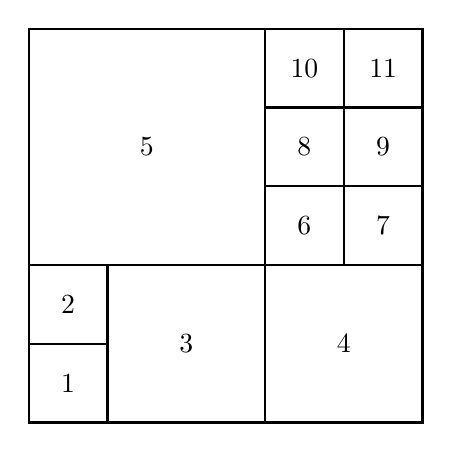
\begin{tikzpicture}[scale=1]
% Draw the outer square
\draw[thick] (0,0) rectangle (5,5);

% Vertical lines
\draw[thick] (1,0) -- (1,2);
\draw[thick] (3,0) -- (3,5);
\draw[thick] (4,2) -- (4,5);

% Horizontal lines
\draw[thick] (0,1) -- (1,1);
\draw[thick] (0,2) -- (5,2);
\draw[thick] (3,3) -- (5,3);
\draw[thick] (3,4) -- (5,4);

% Add labels
\node at (0.5,0.5) {1};
\node at (0.5,1.5) {2};
\node at (2,1) {3};
\node at (4,1) {4};
\node at (1.5,3.5) {5};
\node at (3.5,2.5) {6};
\node at (4.5,2.5) {7};
\node at (3.5,3.5) {8};
\node at (4.5,3.5) {9};
\node at (3.5,4.5) {10};
\node at (4.5,4.5) {11};
\end{tikzpicture}
\end{center}
Prove that all integers greater than 5 are squareable. Hint: Prove by induction with three base cases.

\begin{proof}
We show that $6,7,8$ are squareable:
\begin{center}
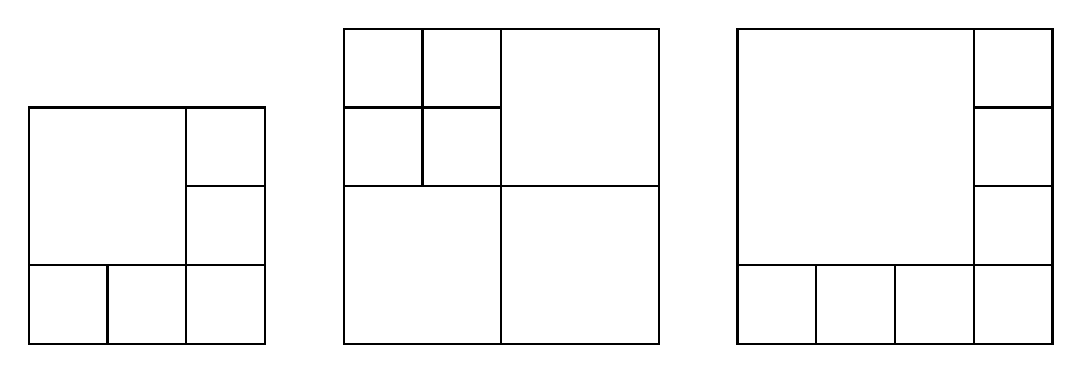
\begin{tikzpicture}[scale=1]

% 6 case
\draw[thick] (0,0) rectangle (3,3);
\draw[thick] (0,1) -- (3,1);
\draw[thick] (1,0) -- (1,1);
\draw[thick] (2,0) -- (2,3);
\draw[thick] (2,2) -- (3,2);

% 7 case
\draw[thick] (4,0) rectangle (8,4);
\draw[thick] (4,3) -- (6,3);
\draw[thick] (4,2) -- (8,2);
\draw[thick] (5,2) -- (5,4);
\draw[thick] (6,0) -- (6,4);

% 8 case
\draw[thick] (9,0) rectangle (13,4);
\draw[thick] (9,1) -- (9,1);
\draw[thick] (10,0) -- (10,1);
\draw[thick] (11,0) -- (11,1);
\draw[thick] (12,0) -- (12,4);
\draw[thick] (9,1) -- (13,1);
\draw[thick] (12,2) -- (13,2);
\draw[thick] (12,3) -- (13,3);

\end{tikzpicture}
\end{center}

Now suppose $n > 8$ and assume by strong induction that all integers $6 \leq k < n$ are squareable. We consider three cases:

\textbf{Case 1:} If $n \equiv 0 \pmod{3}$, then $n = 3k$ for some integer $k \geq 3$. Take any squared tiling of $n-3$ squares and subdivide one square into $4$ equal squares.

\textbf{Case 2:} If $n \equiv 1 \pmod{3}$, then $n = 3k+1$ for some integer $k \geq 2$. Take any squared tiling of $n-3$ squares and subdivide one square into $4$ equal squares.

\textbf{Case 3:} If $n \equiv 2 \pmod{3}$, then $n = 3k+2$ for some integer $k \geq 2$. Take any squared tiling of $n-3$ squares and subdivide one square into $4$ equal squares.

In all cases, $n$ is squareable. By induction, all integers $n \geq 6$ are squareable.
\end{proof}
\end{problem}

\begin{problem}
(**) At a party, prove that the number of people who shook hands an odd number of times is even.

\begin{proof}
Let $E$ be the set of people who shook hands an even number of times, and $O$ be the set of people who shook hands an odd number of times. Let $H$ be the total number of handshakes.

Each handshake involves exactly 2 people, so if we sum up all the handshakes each person made, we count each handshake twice:
\[\sum_{p \in E} (\text{handshakes by } p) + \sum_{p \in O} (\text{handshakes by } p) = 2H.\]

The left side has the form (even) + (sum of $|O|$ odd numbers). For the total to be even, the sum of $|O|$ odd numbers must be even. But a sum of odd numbers is even if and only if there are an even number of them. Therefore $|O|$ is even.
\end{proof}
\end{problem}

\begin{problem}
(**) There exist two positive irrational numbers $s$ and $t$ such that $s^t$ is rational. Hint: Take $s = t = \sqrt{2}$. Prove by cases.
\end{problem}

\begin{problem}
(**) For any positive integer $d$, there exists a number composed only of the digits 7 and 0 such that $d$ divides this number.

\begin{proof}
Consider the $d+1$ numbers:
\[
7, 77, 777, \ldots, \underbrace{777\ldots7}_{d+1 \text{ sevens}}
\]
Denote by $a_n$ the number with $n$ $7$s. At least two must have the same remainder when divided by $d$. This is because there are only $d$ possible remainders $0,1,\ldots,d-1$ but there are $d+1$ numbers.  Let $a_i$ and $a_j$ with $i > j$ have the same remainder modulo $d$. Then:
\[
d \mid (a_i - a_j)
\]
Furthermore,
\begin{align*}
a_i - a_j &= \underbrace{777\ldots7}_{i \text{ sevens}} - \underbrace{777\ldots7}_{j \text{ sevens}} \\
&= \underbrace{777\ldots7}_{j \text{ sevens}}\underbrace{000\ldots0}_{i-j \text{ zeros}}
\end{align*}

This is a number composed only of 7s and 0s, and $d$ divides it.
\end{proof}

\end{problem}

\begin{problem}
(**) What is the minimum number of breaks to break up a chocolate bar made of $m \times n$ little pieces into those very pieces?

\begin{proof}
Every time you break a chocolate bar, you increase the number of pieces by 1. Then you need $mn -1$ breaks no matter what.
\end{proof}
\end{problem}

\end{document}